\documentclass[10pt]{beamer}

\usetheme{metropolis}
\usepackage{appendixnumberbeamer}

\usepackage{booktabs}
\usepackage[scale=2]{ccicons}

\usepackage{pgfplots}
\usepgfplotslibrary{dateplot}

\usepackage{xspace}
\newcommand{\themename}{\textbf{\textsc{metropolis}}\xspace}

\newcommand{\norm}[1]{\left\lVert#1\right\rVert}

% %%%%%%%%%%%%%%%%%%%%%%%%%%%%%%%%%%%%%%%%%%%%%%%%%%%%%%%%%%%%%%%%%%%%%%%%%%%%%

\title{SVM Algorithm}
\subtitle{with Lagrange multipliers and KKT conditions}
\date{\today}
\author{Matteo Conti}
\institute{University of Bologna}
% \titlegraphic{\hfill\includegraphics[height=1.5cm]{logo.pdf}}

% % % % % % % % % % % % % % % % % % % % % % % % % % % % % % % % % % % % % % % %

\begin{document}

\maketitle

\begin{frame}{Table of contents}
  \setbeamertemplate{section in toc}[sections numbered]
  \tableofcontents[hideallsubsections]
\end{frame}

% %%%%%%%%%%%%%%%%%%%%%%%%%%%%%%%%%%%%%%%%%%%%%%%%%%%%%%%%%%%%%%%%%%%%%%%%%%%%%

\section{Problem Formulation}
\begin{frame}[fragile]{Our Problem}
  \begin{columns}[onlytextwidth, T, c]
    \begin{column}{.5\textwidth}
      initial constrainted problem:
      \newline
      \begin{equation*}
        \begin{split}
          \text{min}\ &\ \frac{1}{2} \norm{w}^2 \\
          \text{s.t.}\ &\ \forall_{i}\ y_i (x_i \cdot w + b) -1 \geq 0
        \end{split}
      \end{equation*}
    \end{column}
    \begin{column}{.5\textwidth}
        \begin{figure}
          \centering    
          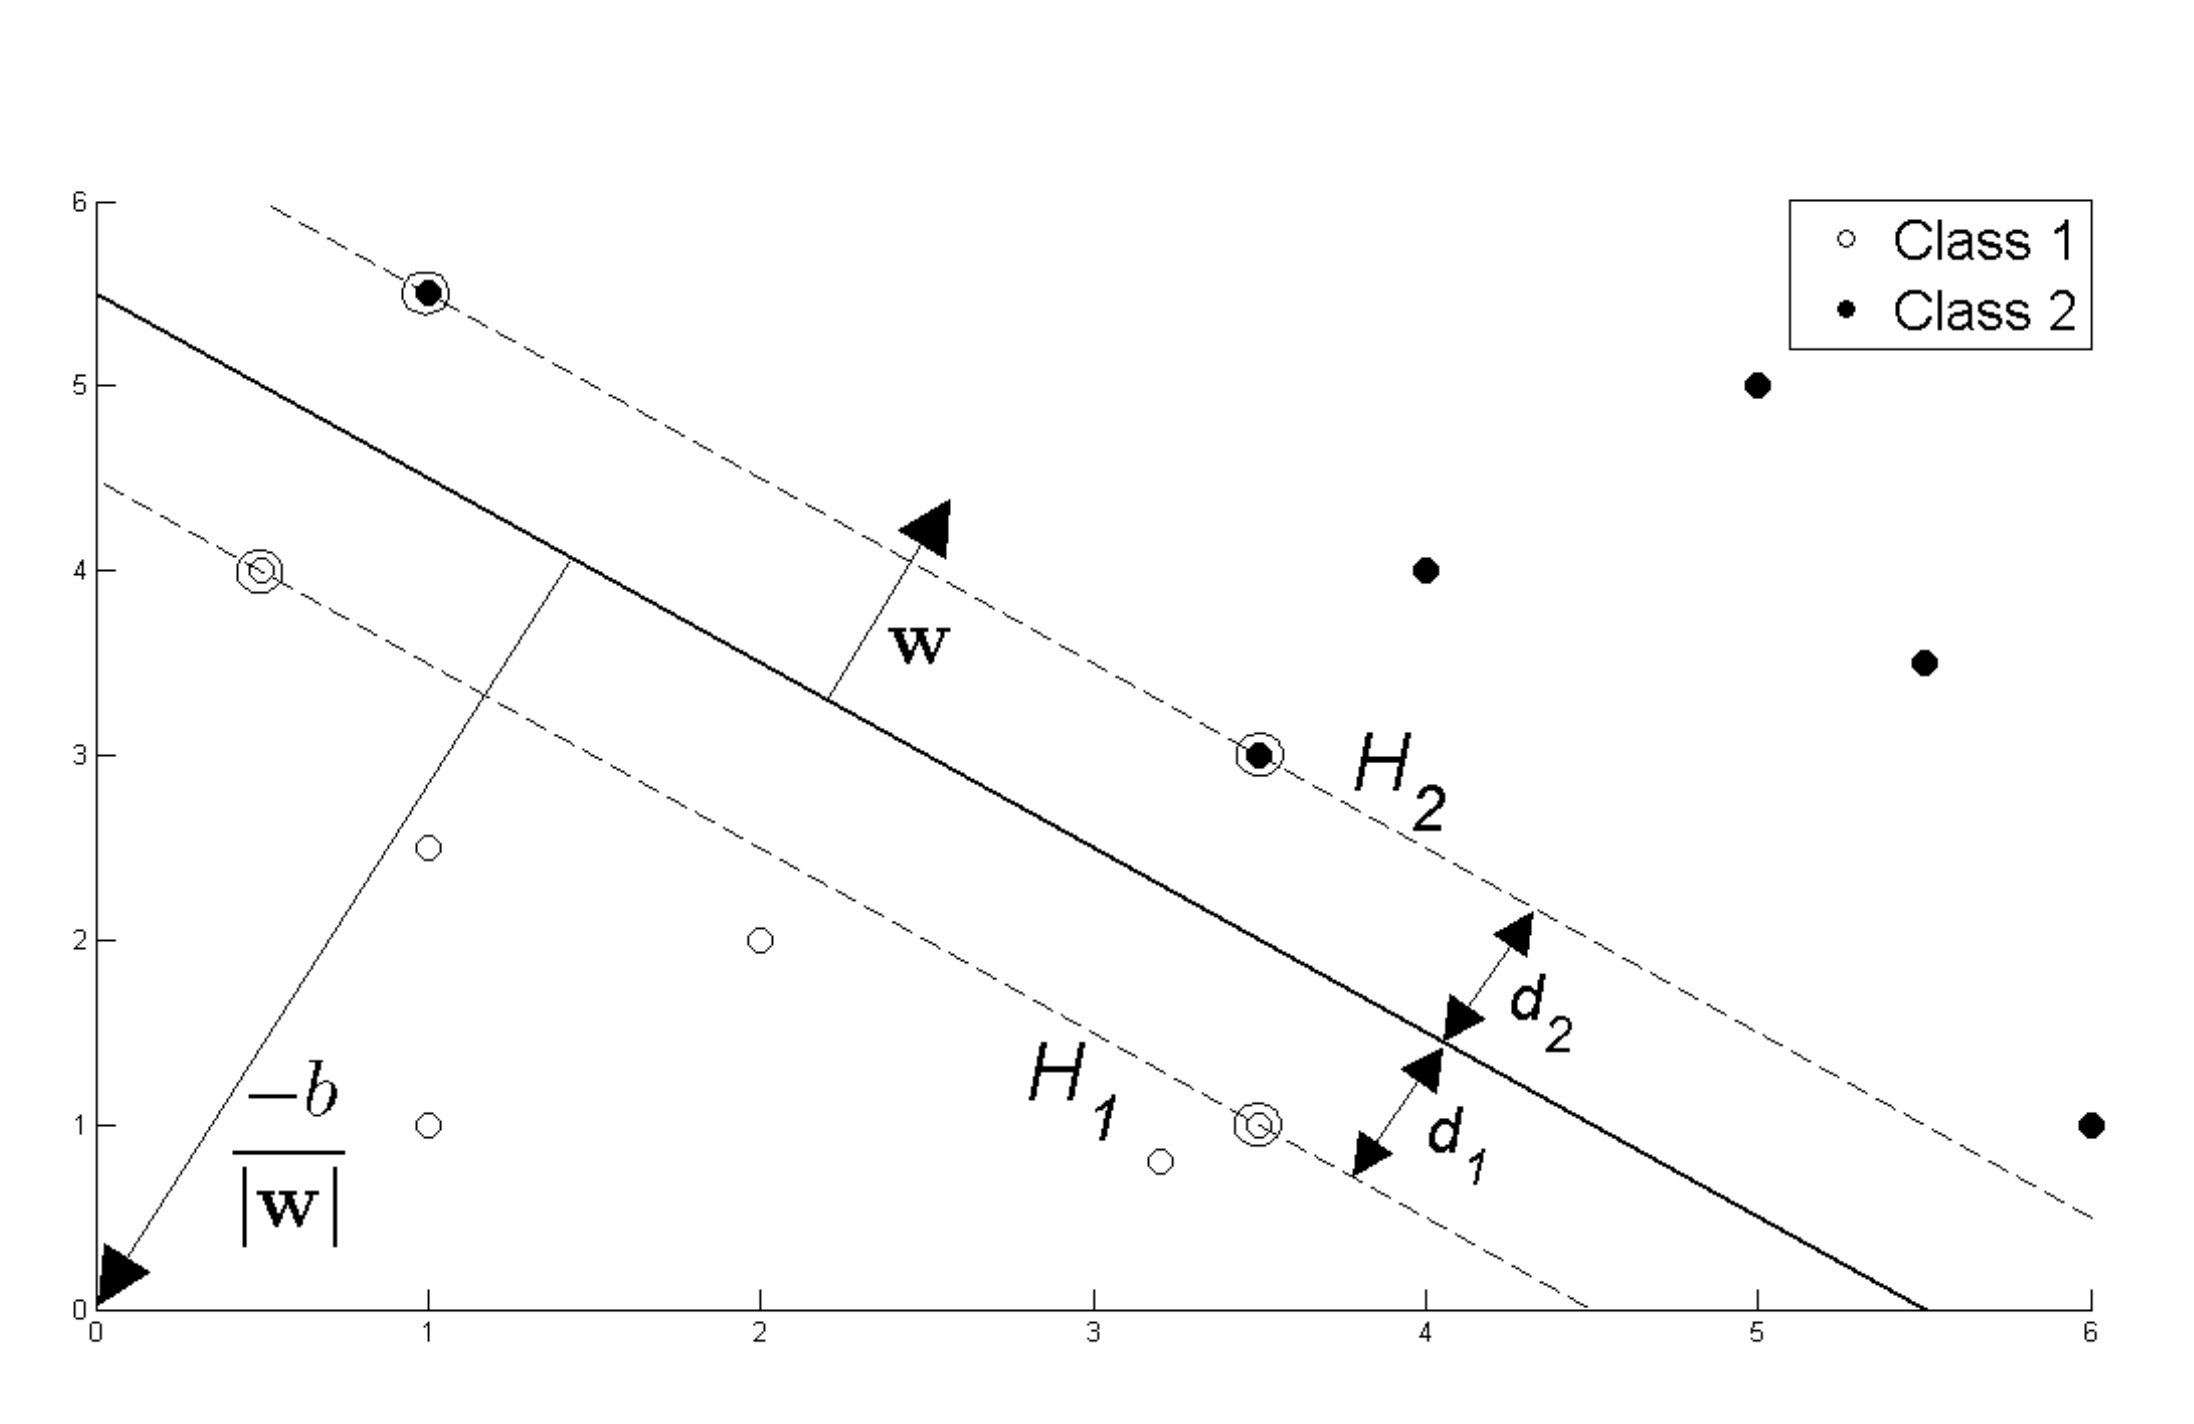
\includegraphics[width=5cm]{assets/images/s1.01.png}
        \end{figure}
    \end{column}    
  \end{columns}
  
  \vspace{.7cm}
  
  % where the hyperplane equation is $w \cdot x + b = 0$
  % and the perpendicular distance from the hyperplane to the origin is $\frac{b}{\norm{w}}$
  the points (circled) $H1$ and $H2$ that lie closest to the separating hyperplane, 
  i.e. the \textbf{Support Vectors}, can be described by
  \begin{equation*}
    \begin{split}
      x_i \cdot w + b = +1 & \hspace{.5cm} \text{for} \hspace{.5cm} H1 \\
      x_i \cdot w + b = -1 & \hspace{.5cm} \text{for} \hspace{.5cm} H2
    \end{split}
  \end{equation*}

\end{frame}


\begin{frame}[fragile]{Lagrangian Multipliers Strategy}
  we formulate our problem as:
  \newline
  \begin{equation*}
    \begin{split}
      L_P\ \equiv\ \frac{1}{2} \norm{w}^2 - \alpha [\forall_i\  y_i (x_i \cdot w + b) - 1]
    \end{split}
  \end{equation*}

  where $\alpha_i$ are the Lagrange \textbf{multipliers} such that:
  \begin{equation*}
    \forall_i\ \alpha_i\ \geq 0 
  \end{equation*}

  we want to \textbf{min} $L_P(w,b)$ and then \textbf{max} $L_P(\alpha)$.
\end{frame}


\begin{frame}[fragile]{Final Problem Formulation}
  Dual form of the primary Lagrangian problem:
  \newline
  \begin{equation*}
    \begin{split}
      \max_{\alpha}\ &\ L_D\ \equiv\ \sum_{i=1}^{L} \alpha_i - \frac{1}{2} \sum_{i,j} \alpha_i \alpha_j y_i y_j x_i \cdot x_j
      \equiv\ \sum_{i=1}^{L} \alpha_i - \frac{1}{2} \alpha^T H \alpha
    \end{split}
  \end{equation*}

  where:
  \newline
  \begin{equation*}
    H\ \equiv\ y_i y_j x_i \cdot x_j
  \end{equation*}

  subject to:
  \newline
  \begin{equation*}
    \sum_{i=1}^{L} \alpha_i y_i = 0 \hspace{.5cm} \text{and} 
    \hspace{.5cm} 
    \forall_i\ \alpha_i \geq 0 
  \end{equation*}
\end{frame}


% % % % % % % % % % % % % % % % % % % % % % % % % % % % % % % % % % % % % % % %

\section{Quadratic-Programming Optimization}
\begin{frame}[fragile]{Quadratic-Programming Solver}
  We have used the \emph{cvxopt} Python library in order to obtain the 
  solutions for our Quadratic-Programming problem.
  \vspace{.5cm}

  This library solve a problem in the form
  \begin{equation*}
    \begin{split}
      \min_{x}\ &\ \ \frac{1}{2} x^T P x + q^T x \\
          s.t.\ &\ \ Gx \leq h \\
              \ &\ \ Ax = b
    \end{split}
  \end{equation*}
  \vspace{.5cm}

  So we've ended up in adapting our $max_{x}\ L_D$ problem to the above formulation
  in order to find $\alpha_i$ solutions (look at the code for more details).
\end{frame}


% % % % % % % % % % % % % % % % % % % % % % % % % % % % % % % % % % % % % % % %

\section{Soft-Margin Assumption}
\begin{frame}[fragile]{Soft-Margin Assumption}
  \textcolor{lightgray}{Dual form of the primary Lagrangian problem:}
  \newline
  \begin{equation*}
    \begin{split}
      \textcolor{lightgray}{\max_{\alpha}\ \sum_{i=1}^{L} \alpha_i - \frac{1}{2} \alpha^T H \alpha}
    \end{split}
  \end{equation*}

  subject to:
  \newline
  \begin{equation*}
    \textcolor{lightgray}{\sum_{i=1}^{L} \alpha_i y_i = 0 \hspace{.5cm} \text{and}}
    \hspace{.5cm} 
    \textcolor{blue}{\forall_i\ \mathbf{C \geq \alpha_i \geq 0}}
  \end{equation*}

  \vspace{.3cm}

  where $\mathbf{C}$ controls the trade-off between the slack variable penalty 
  and the size of the margin (a low $\mathbf{C}$ makes the hyperplane decision 
  surface smooth, while a high $\mathbf{C}$ aims at classifying all points correctly).
\end{frame}

\begin{frame}[fragile]{Hard-Margin vs Soft-Margin}
  \begin{columns}[onlytextwidth, T, c]
    \begin{column}{.5\textwidth}
        \begin{figure}
            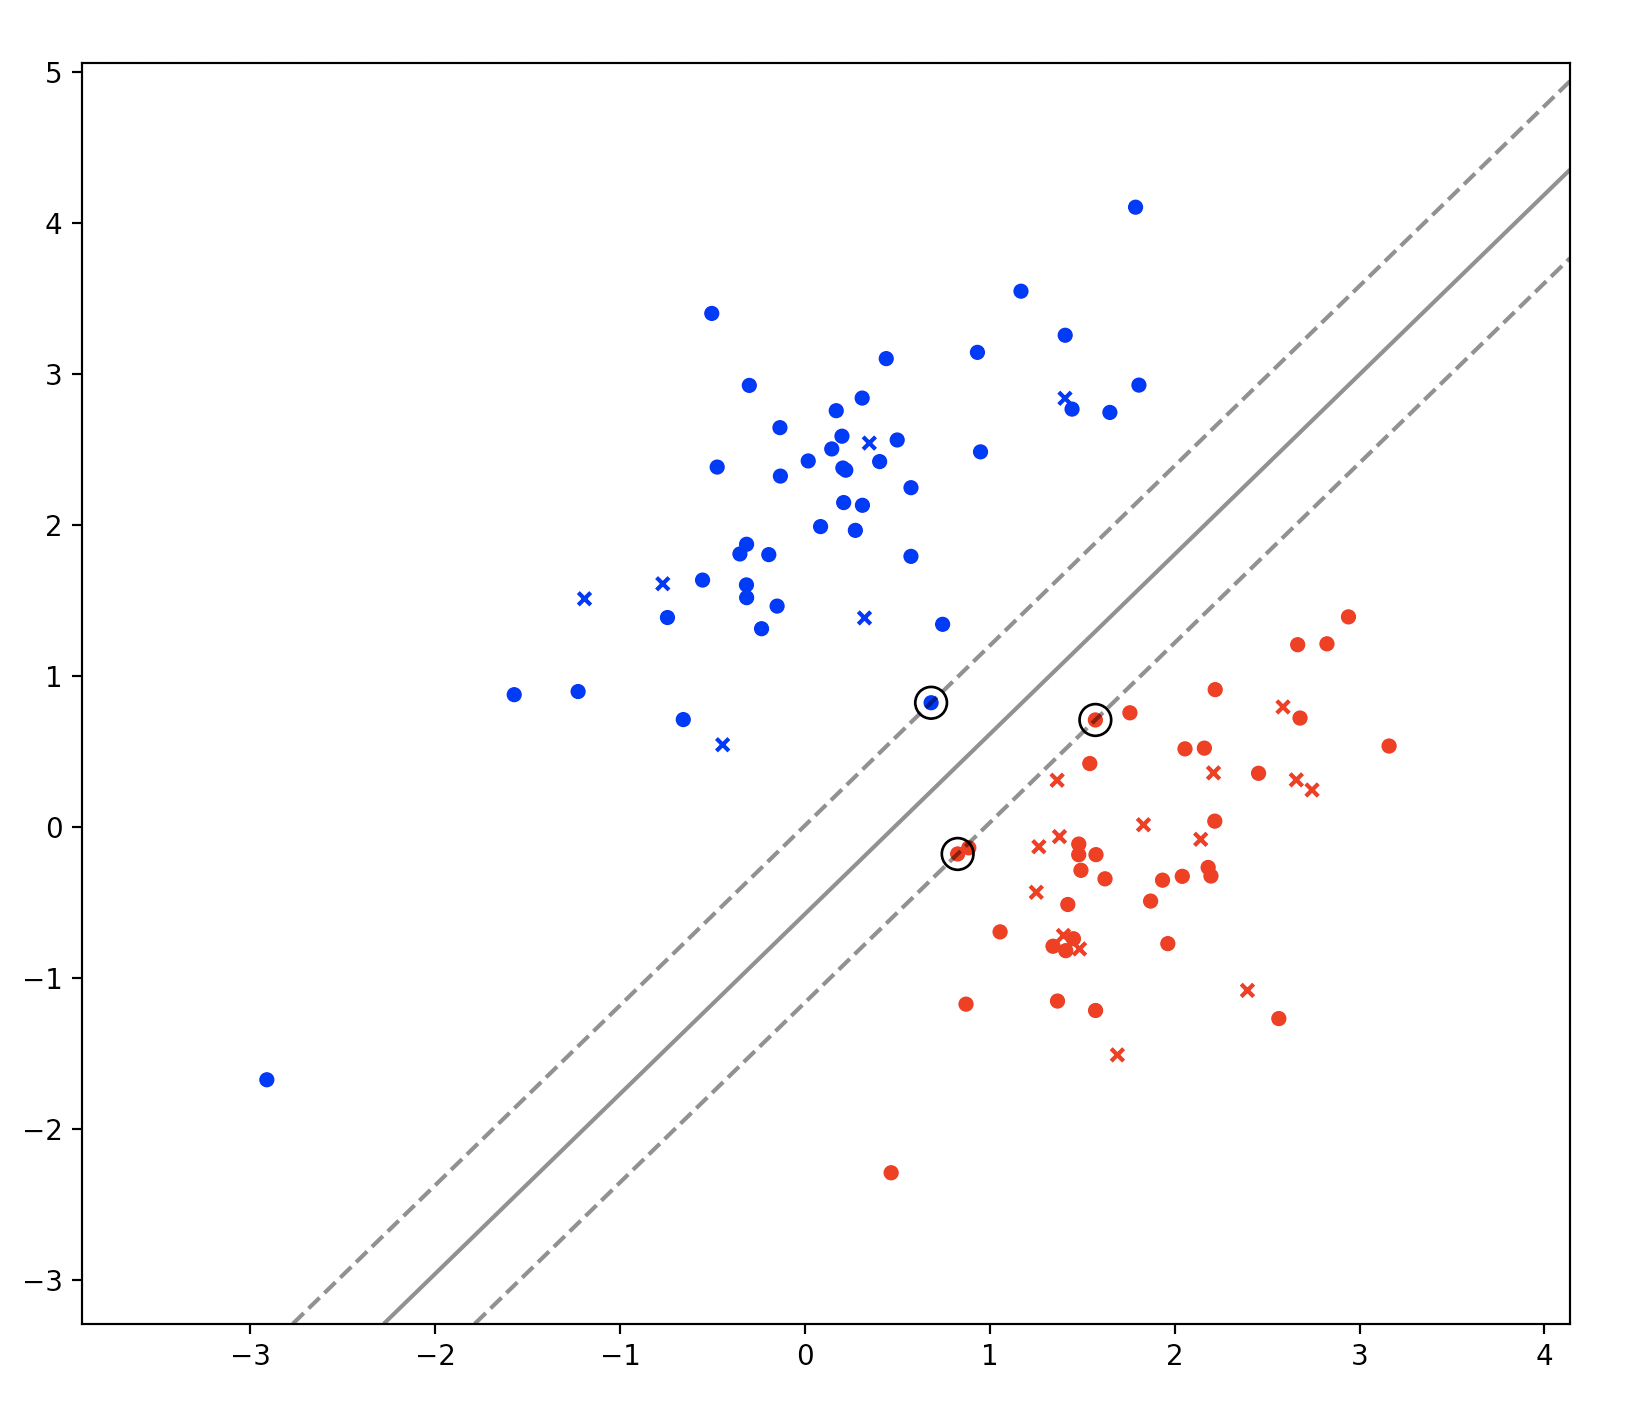
\includegraphics[width=5cm]{assets/images/s3.01.png}
            \caption{Hard-Margin}
        \end{figure}
    \end{column}
    \begin{column}{.5\textwidth}
        \begin{figure}
            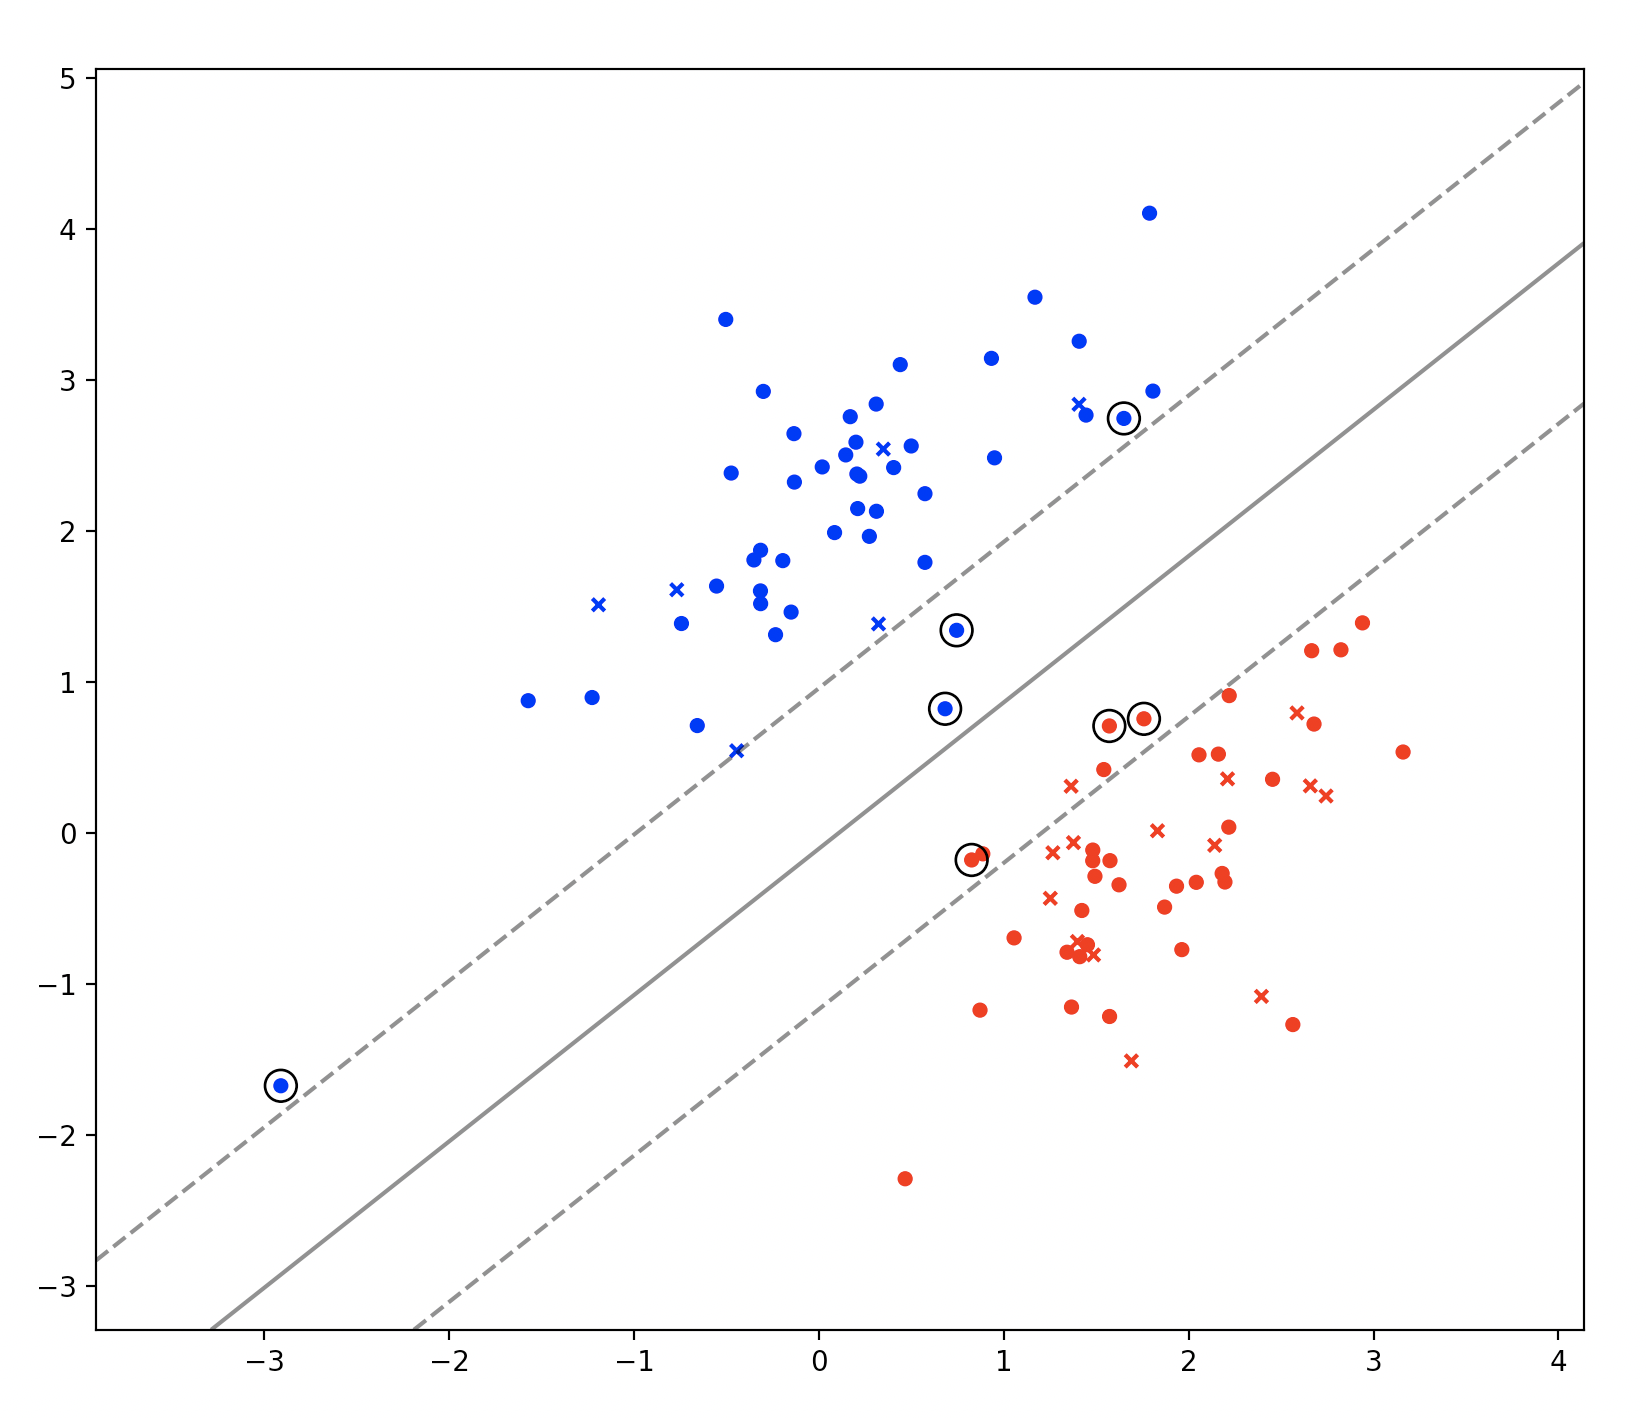
\includegraphics[width=5cm]{assets/images/s3.02.png}
            \caption{Soft-Margin}
        \end{figure}
    \end{column}    
  \end{columns}
\end{frame}


% % % % % % % % % % % % % % % % % % % % % % % % % % % % % % % % % % % % % % % %

\section{Non-Linear Kernel}
\begin{frame}[fragile]{Non-Linear Kernel}
  Dual form of the primary Lagrangian problem:
  \newline
  \begin{equation*}
    \begin{split}
      \textcolor{blue}{\max_{\alpha}}\ &\ \textcolor{blue}{L_D}\ 
      \equiv\ 
      \textcolor{lightgray}{\sum_{i=1}^{L} \alpha_i - \frac{1}{2} \alpha^T} 
      \mathbf{\textcolor{blue}{H}}
      \textcolor{lightgray}{\alpha}
    \end{split}
  \end{equation*}

  where:
  \newline
  \begin{equation*}
    \textcolor{blue}{H}\ \equiv\ \textcolor{lightgray}{y_i y_j} \mathbf{\textcolor{blue}{k(x_i, x_j)}}
  \end{equation*}

  linear kernel is defined as:
  \begin{equation*}
    k(x_i, x_j) = \phi(x_i) \cdot \phi(x_j)
  \end{equation*}

  polynomial kernel is defined as:
  \begin{equation*}
    k(x_i, x_j) = (\phi(x_i) \cdot \phi(x_j) + 1)^{deg}
  \end{equation*}
\end{frame}

\begin{frame}[fragile]{Non-Linear Kernel}
  \begin{columns}[onlytextwidth, T, c]
    \begin{column}{.5\textwidth}
        \begin{figure}
            % TODO: ...
            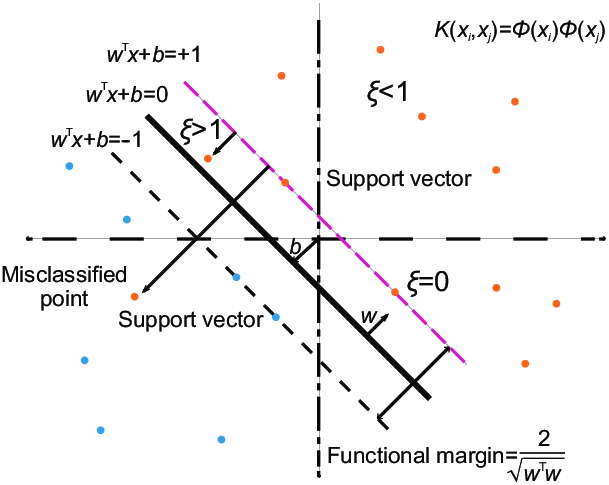
\includegraphics[width=5cm]{assets/images/test.png}
            \caption{Linear Kernel}
        \end{figure}
    \end{column}
    \begin{column}{.5\textwidth}
        \begin{figure}
            % TODO: ...
            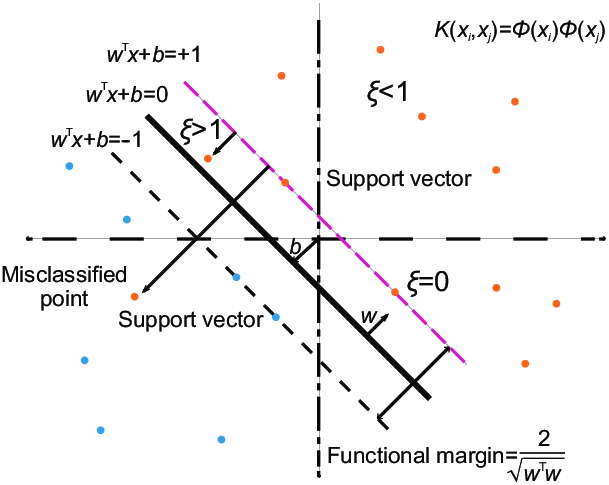
\includegraphics[width=5cm]{assets/images/test.png}
            \caption{Polynomial Kernel}
        \end{figure}
    \end{column}    
  \end{columns}
\end{frame}


% % % % % % % % % % % % % % % % % % % % % % % % % % % % % % % % % % % % % % % %

\begin{frame}[standout]
  \small{\emph{www.github.com/contimatteo/SVM-from-scratch}}
\end{frame}

% %%%%%%%%%%%%%%%%%%%%%%%%%%%%%%%%%%%%%%%%%%%%%%%%%%%%%%%%%%%%%%%%%%%%%%%%%%%%%

\end{document}
